\chapter{Specyfikacja wewnętrzna}
\label{ch:05}

\section{Przedstawienie idei}
Celem aplikacji, jest umożliwienie wielu użytkownikom wspólnego zarządzania listą odtwarzania utworów. Aby to osiągnąć wykorzystane zostało API serwisu Spotify, które umożliwia ingerencję w konto użytkownika, który wyraził na to zgodę (logując się do systemu). Dzięki udostępnionym funkcjom aplikacja ma dostęp do bazy utworów serwisu, możliwe jest także sterowanie odtwarzaczem muzyki, w tym dodawanie utworów do kolejki odtwarzania. Po poprawnym zalogowaniu przez użytkownika Spotify system zapisuje w bazie jego tokeny umożliwiające dostęp do zapytań, które ingerują w jego konto. W momencie, kiedy gość sesji doda utwór do kolejki, aplikacja serwera używając odpowiednich tokenów dodaje utwór w imieniu właściciela.

Aby zapewnić prostotę używania aplikacji, system nie wymaga od gości sesji rejestracji, a jedynie podania poprawnego kodu oraz pseudonimu. Serwer w odpowiedzi na udaną autoryzację odsyła token dostępu, bez którego wszystkie zapytania, które nie należą do punktu końcowego autoryzacji zostaną odrzucone. Tokeny dostępu mają datę ważności, po której przestają działać a konto zostaje dezaktywowane, użytkownik musi się wtedy ponownie uwierzytelnić.


\section{Architektura systemu}
Zgodnie z wielowarstwowym modelem aplikacji internetowej system składa się z 3 osobnych elementów:
\subsection{Warstwa danych}
Warstwa odpowiedzialna za przetrzymywanie oraz pozyskiwanie danych została zrealizowana przy pomocy gotowych już narzędzi. Serwer, na którym działa silnik bazy danych (PostgreSQL) obsługuje zapytania SQL. W trakcie implementacji serwer bazy danych został utworzony lokalnie na maszynie wirtualnej przy pomocy narzędzia Docker. Interakcję z bazą danych implementuje mechanizm dostępny jako moduł szkieletu Spring. Udostępnia on przejrzysty i łatwy w obsłudze interfejs programistyczny, który wprowadza pewną warstwę abstrakcji, aby ułatwić realizację interakcji z bazą danych.

\subsection{Warstwa usług}
Część systemu realizująca logikę biznesową została zaimplementowana korzystając ze szkieletu programistycznego Spring oraz języka Java. Aplikacja implementuje architekturę opartą na wzorcu model-widok-kontroler, natomiast warstwa widoku została zrealizowana w osobnej aplikacji. Dodatkowo istnieje jeszcze warstwa zapewniająca bezpieczeństwo systemu.

Po otrzymaniu zapytania przez serwer trafia ono do łańcucha filtrów, które sekwencyjnie sprawdzają żądanie między innymi w celach bezpieczeństwa. W aplikacji zaimplementowane zostały dwa filtry, które sprawdzają tożsamość użytkownika (uwierzytelnianie) na podstawie tokenu JWT obecnego w nagłówku żądania. Kolejnym etapem jest autoryzacja, czyli potwierdzenie czy uwierzytelniony użytkownik ma dostęp do zasobu, którego żąda. Następnie żądanie jest mapowane do odpowiedniego kontrolera, który wywołuje odpowiednie serwisy implementujące logikę biznesową. Serwisy korzystają z repozytoriów, których głównym zadaniem jest komunikacja z bazą danych. Dodatkowo wykorzystują inne serwisy, które przykładowo realizują połączenie z zewnętrznym API platformy Spotify. Otrzymane wyniki są odpowiednio przetwarzane przez serwisy i zwracane do kontrolera, który odsyła odpowiedź do klienta. Serwisy stanowią część modelu aplikacji.

\subsection{Warstwa prezentacji}
Jest to część systemu odpowiedzialna za interakcję z użytkownikiem, została zaimplementowana przy użyciu szkieletu programistycznego Angular oraz języka TypeScript. Aplikacja została utworzona w architekturze SPA co oznacza, że aplikacja raz pobrana z serwera WWW nie wymaga przeładowania w celu zmiany wyświetlanych treści, lecz jest to wykonywane asynchronicznie w tle. Aplikacja składa się z komponentów, które reprezentują każdą część interfejsu użytkownika i realizują daną funkcjonalność oraz określają styl i rozmieszczenie poszczególnych elementów. Przykładowo komponent, który implementuje funkcjonalność odtwarzacza muzyki, może być ponownie używany w innych komponentach bez konieczności niepotrzebnego powtarzania kodu. Komponenty korzystają z serwisów, których zadaniem jest komunikacja z warstwą usług. Serwisy udostępniają funkcje, które odpowiednio tworzą, wysyłają oraz odbierają zapytania. Obiekty, które uczestniczą w wymianie między warstwą prezentacji a warstwą usług są zdefiniowane w modelu aplikacji.

\section{Organizacja bazy danych}
Aby zrealizować założenia projektu konieczne było zaprojektowanie oraz implementacja bazy danych. Diagram przedstawiony na Rys. \ref{fig:database} pokazuje jakie relacje zachodzą między poszczególnymi tabelami. W centrum diagramu widnieje kluczowy element systemu - sesja, przechowuje ona podstawowe informacje takie jak data utworzenia czy kod dostępu oraz nazwę. Sesja jest ściśle powiązana z tabelą właścicieli, gdzie właściciel może posiadać wiele sesji natomiast sesja tylko jednego właściciela. Tabela właścicieli przechowuje informacje niezbędne do komunikacji z zewnętrznym API platformy Spotify - tokeny dostęp oraz nazwę i id użytkownika w serwisie. Ustalone zasady sesji są unikatowe dla każdej sesji i przechowują informację o ustalonych przez właściciela wartościach takich jak maksymalna ilość utworów, które może dodać gość czy maksymalna ilość gości w sesji oraz czy dozwolone będą utwory oznaczone jako zawierające treści dla dorosłych i czy powinna zostać utworzona lista z dodanymi utworami. W bazie danych przetrzymywane są także informacje o gościach, którzy dołączyli do sesji takie jak ilość dodanych przez nich utworów oraz pseudonim, który ustawili dołączając do sesji. Gość może należeć tylko do jednej sesji, natomiast w sesji może znajdować się wielu gości. Baza danych zawiera także informacje o tym jakie utwory zostały dodane do kolejki w danej sesji oraz jakie gatunki utworów właściciel zablokował, funkcjonalność ta jest obecnie dostępna jedynie z poziomu API aplikacji i nie jest możliwa do ustawienia używając interfejsu użytkownika.


\section{Użyte biblioteki}
\begin{itemize}
\item Lombok - biblioteka generująca powtarzalny i rutynowy kod taki jak konstruktor czy metody pobierające i ustawiające wartości obiektu poprzez użycie odpowiednich adnotacji, co poprawia czytelność kodu. 

\item io.jsonwebtoken - biblioteka obsługująca tokeny JWT, za pomocą której możliwe jest tworzenie, walidacja oraz parsowanie tokenów dostępu.

\item ZXing - biblioteka umożliwiająca generowanie kodów QR.

\item Jakarta Bean Validation - narzędzie służące do walidacji danych, poprzez odpowiednie adnotacje, dzięki czemu reguły dotyczące pól obiektów są wyraźnie zdefiniowane.

\item ngx-cookie-service - moduł biblioteki obsługującej pliki cookie, w których trzymany jest token dostępu po autoryzacji użytkownika.
\end{itemize}

\section{Ważniejsze klasy}
\begin{itemize}
\item Interfejsy kontrolerów API

Są to automatycznie wygenerowane klasy przez narzędzie OpenAPI generator. Tworzą one szkielet aplikacji i definiują sygnatury metod, które należy zaimplementować. Każda z funkcji opatrzona jest odpowiednimi adnotacjami, które określają ścieżkę, parametry oraz ich walidację, metody autoryzacji, rodzaj żądania odpowiadającemu danemu punktowi końcowymi itp.

\item Serwisy

Klasy implementujące logikę biznesową korzystając z innych serwisów oraz bazy danych poprzez metody udostępniane przez repozytoria. Każda klasa implementuje odpowiedni interfejs aby zapewnić niezależność między deklaracją metod a ich implementacją. Większość serwisów dodatkowo mapuje otrzymane wyniki na obiekty, które uczestniczą w komunikacji z klientem.

\item Klasa do generacji kodów dostępu i kodów QR

Generowanie nowych kodów dostępu odbywa się podczas tworzenia nowych sesji. Na Rys. \ref{fig:code-generation} przedstawiony jest kod, który jest za to odpowiedzialny. Z tablicy dozwolonych znaków w sposób losowy wybrane jest kolejno 6 znaków. Kluczowa tutaj jest klasa SecureRandom, która jest dużo bardziej bezpieczna pod względem kryptografii. Do generacji liczby losowej wykorzystane jest kilka źródeł losowości takich jak ruch sieciowy, ruch dyskowy czy czas systemowy. 

\begin{figure}[h]
\centering
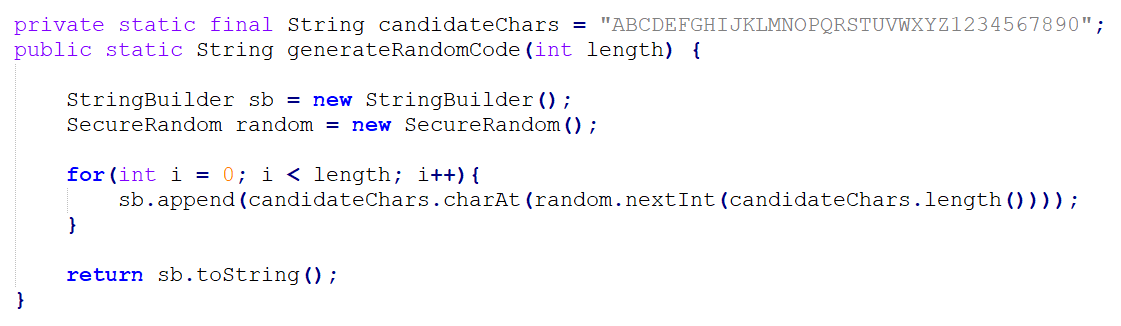
\includegraphics[width=0.9\textwidth]{./graf/code_generation.PNG}
\caption{Fragment kodu - generowanie losowych kodów dostępu}
\label{fig:code-generation}
\end{figure}

\end{itemize}
\section{Szczegóły implementacji}
\subsection{Zastosowane wzorce projektowe}
\begin{itemize}
\item Pełnomocnik

Aby zapewnić kontrolę dostępu do danych z serwisu Spotify oraz dalszą ich modyfikację i korzystanie z nich w logice biznesowej zastosowany został wzorzec pełnomocnika. Oznacza to, że otrzymane wyniki zanim zostaną zwrócone do klienta są dodatkowo modyfikowane i używane w implementacji logiki, aby przykładowo sprawdzić czy utwór, który użytkownik chciał dodać spełnia zasady sesji. Dodatkowo chronione są dzięki temu dane użytkowników Spotify, ponieważ ich tokeny dające dostęp do niektórych funkcjonalności konta w serwisie nie są nigdy udostępniane na zewnątrz.

\item Model-Widok-Kontroler

Zastosowany został podział, który rozdziela logikę od wyglądu w systemie, zapewniając jednocześnie niezależność obu komponentów co pozwala dowolnie zmieniać ich sposób realizacji. Komunikację między modelem a widokiem zapewnia kontroler.

\item Architektura wielowarstwowa (dokładnie trójwarstwowa)

Zastosowany został podział, dzielący system na trzy warstwy: prezentację, czyli interfejs użytkownika, logikę biznesową oraz dane. Każdy z wymienionych modułów to osobna aplikacja, dzięki czemu zachowana jest niezależność.

\item Wstrzykiwanie zależności

Mechanizmy szkieletu programistycznego Spring implementują ten wzorzec, aby przekazywać zależności między obiektami w prosty sposób bez konieczności ingerencji w przekazywany komponent. Zależności są dostarczane do obiektu co poprawia łatwość utrzymania aplikacji.
\end{itemize}
\section{Diagramy UML}

\begin{figure}[h]
\centering
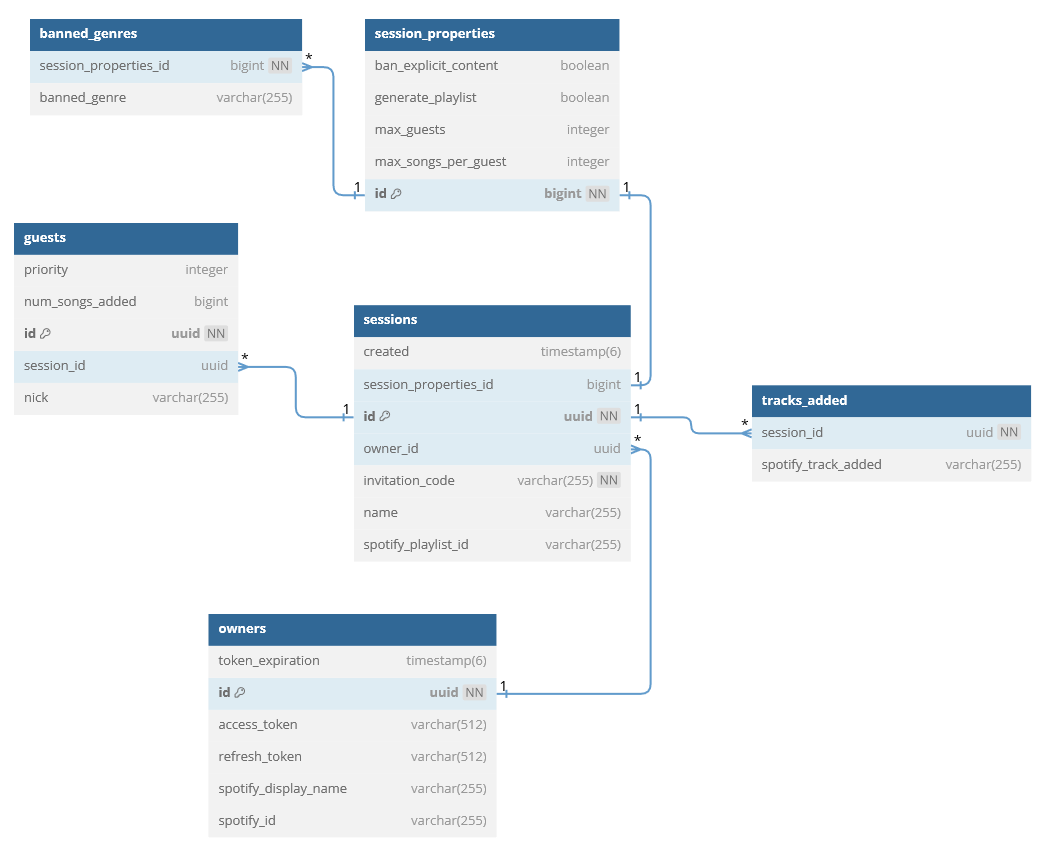
\includegraphics[width=1.0\textwidth]{./graf/database_diagram.png}
\caption{Diagram modelu bazy danych}
\label{fig:database}
\end{figure}



